
\section{Elementos Visuais}
O projeto bebe de variadas fontes de inspirações, e planeja levar o jogador para o ambiente em que os personagem que ele irá controlar vivem, finalizando em outro ambiente que misturará elementos de todos os ambientes.


Todos os personagens foram baseados em estatuetas artesanais, desenhados em 2D e por fim modelados em 3D.

\subsection{Duende}
\begin{figure}[htb]
	\caption{\label{duendeRef}Estatueta de Duende}
	\begin{center}
	    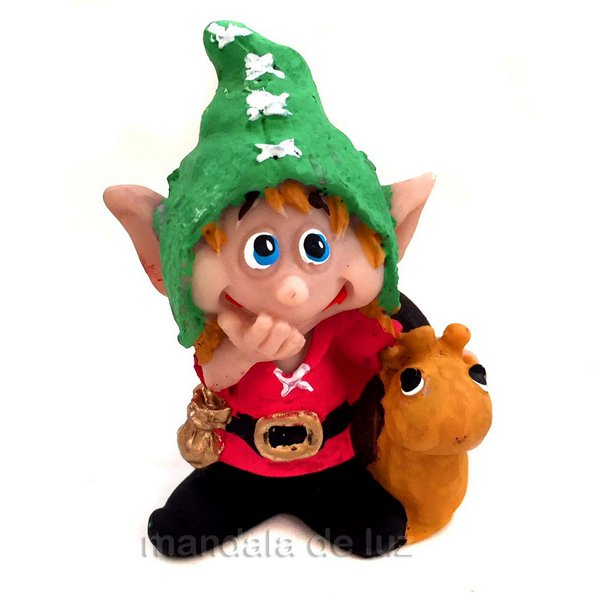
\includegraphics[width=\textwidth/2]{imagens/duendeRef.jpg}
	\end{center}
	\legend{Fonte: (Mandala de Luz, 2012)}
\end{figure}



\begin{figure}[htb]
	\caption{\label{duendePos}Arte Conceitual Duende}
	\begin{center}
	    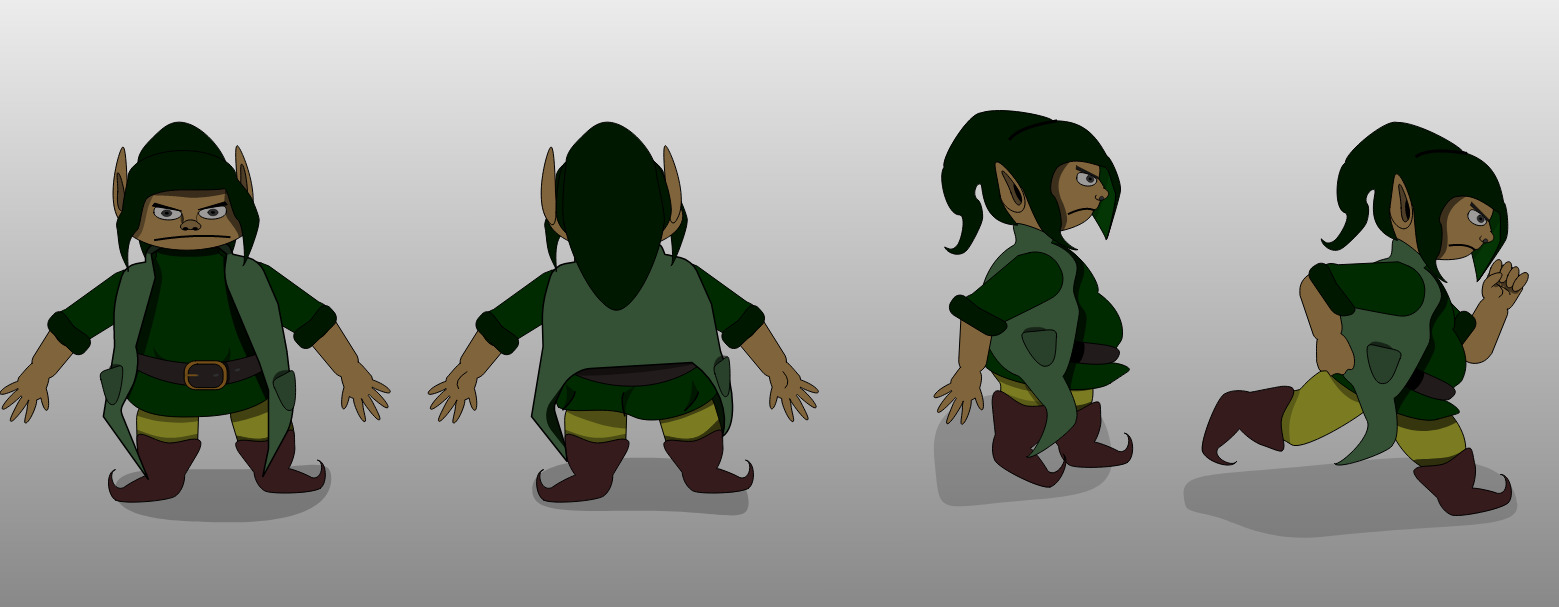
\includegraphics[width=\textwidth]{imagens/duendePosicoes.jpeg}
	\end{center}
	\legend{Fonte: Autoria Própria - Marina Araujo}
\end{figure}

\clearpage

\subsection{Xamã}

\subsection{Bruxa}

\subsection{Ogof}
\begin{figure}[htb]
	\caption{\label{mago}mago}
	\begin{center}
	    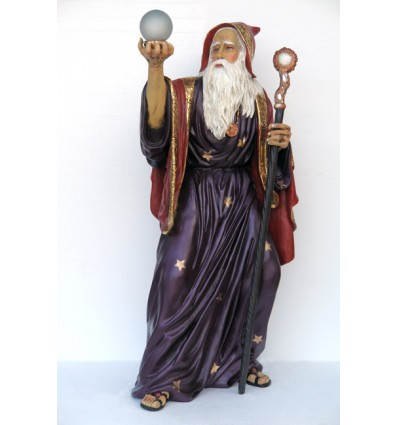
\includegraphics[width=\textwidth/2]{imagens/mago.jpg}
	\end{center}
	\legend{Fonte: (Macocaya, 2010)}
\end{figure}

\begin{figure}[htb]
	\caption{\label{Ogof}Ogof}
	\begin{center}
	    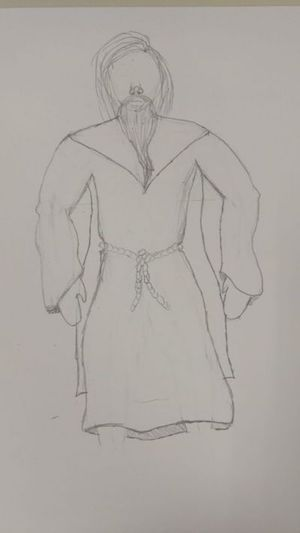
\includegraphics[width=\textwidth/2]{imagens/Ogof.jpg}
	\end{center}
	\legend{Fonte: Autoria Própria - Marina Araujo}
\end{figure}

\clearpage

\subsection{Paleta de cores}
\begin{figure}[htb]
	\caption{\label{paleta}paleta}
	\begin{center}
	    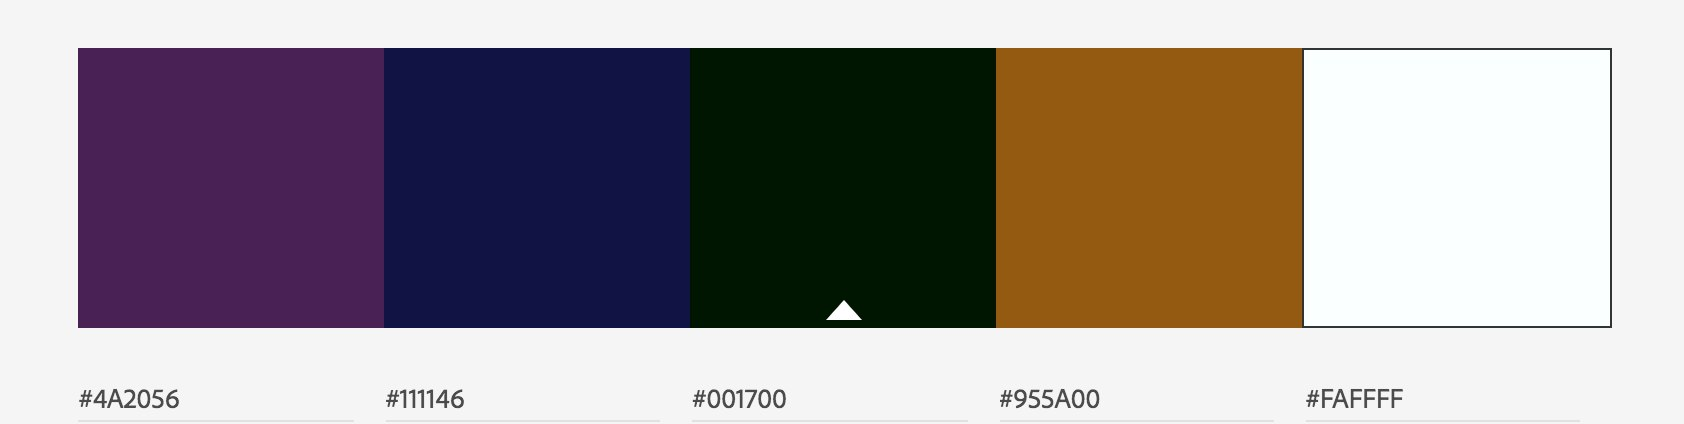
\includegraphics[width=\textwidth/2]{imagens/paleta.jpg}
	\end{center}
	\legend{Fonte: Própria Autoria}
\end{figure}

\section{Elementos Sonoros}

Descreva os elementos chave; como estão sendo desenvolvidos; qual o estilo musical. Inclua detalhes sobre efeitos sonoros e inspirações.
